\iffalse
\documentclass[12pt]{article}
\usepackage{graphicx}
\usepackage[none]{hyphenat}
\usepackage{graphicx}
\usepackage{listings}
\usepackage[english]{babel}
\usepackage{graphicx}
\usepackage{caption} 
\usepackage{booktabs}
\usepackage{array}
\usepackage{amssymb} % for \because
\usepackage{amsmath}   % for having text in math mode
\usepackage{extarrows} % for Row operations arrows
\usepackage{listings}
\lstset{
  frame=single,
  breaklines=true
}
\usepackage{hyperref}
  
%Following 2 lines were added to remove the blank page at the beginning
\usepackage{atbegshi}% http://ctan.org/pkg/atbegshi
\AtBeginDocument{\AtBeginShipoutNext{\AtBeginShipoutDiscard}}
\usepackage{gensymb}


%New macro definitions
\newcommand{\mydet}[1]{\ensuremath{\begin{vmatrix}#1\end{vmatrix}}}
\providecommand{\brak}[1]{\ensuremath{\left(#1\right)}}
\providecommand{\norm}[1]{\left\lVert#1\right\rVert}
\providecommand{\abs}[1]{\left\vert#1\right\vert}
\newcommand{\solution}{\noindent \textbf{Solution: }}
\newcommand{\myvec}[1]{\ensuremath{\begin{pmatrix}#1\end{pmatrix}}}
\let\vec\mathbf


\begin{document}

\begin{center}
\title{\textbf{Tangents and Normals}}
\date{\vspace{-5ex}} %Not to print date automatically
\maketitle
\end{center}
\setcounter{page}{1}

\section{12$^{th}$ Maths - Chapter 6}
This is Problem-2 from Exercise 6.3 
\begin{enumerate}
\fi
\begin{enumerate}
\item The given equation of the curve can be rearranged as
\begin{align}
	xy-x-2y+1 &= 0 \\
        \label{eq:chapters/12/6/3/2/Eq1}
	\implies \vec{x}^\top\myvec{0 & \frac{1}{2} \\ \frac{1}{2} & 0}\vec{x} + \myvec{-1 & -2}\vec{x}+1 &= 0 
\end{align}
The above equation can be equated to the generic equation of conic sections
\begin{align}
	\label{eq:chapters/12/6/3/2/Eq2}
	g\brak{\vec{x}} = \vec{x}^T\vec{V}\vec{x} + 2\vec{u}^T\vec{x} + f = 0 
\end{align}
Comparing coefficients of both equations \eqref{eq:chapters/12/6/3/2/Eq1} and \eqref{eq:chapters/12/6/3/2/Eq2} 
\begin{align}
	\vec{V} &= \myvec{ 0 & \frac{1}{2} \\ \frac{1}{2} & 0} \\
	\vec{u} &= -\myvec{\frac{1}{2} \\ 1} \\
	f &= 1 
\end{align}
Given the point of contact $\vec{q}$, the normal vector of the tangent to \eqref{eq:chapters/12/6/3/2/Eq2} is
\begin{align}
	\label{eq:chapters/12/6/3/2/Eq3}
        \kappa \vec{n} = \vec{V}\vec{q}+\vec{u}, \kappa \in \mathbb{R}
\end{align}
For the given point of contact with $\vec{q}_1=10$,
\begin{align}
	\vec{q}_2 = \frac{10-1}{10-2} = \frac{9}{8} \\
	 \therefore \vec{q} = \myvec{10 \\ \frac{9}{8}}
\end{align}
\begin{align}
	& \eqref{eq:chapters/12/6/3/2/Eq3} \implies  \kappa \vec{n} = \myvec{ 0 & \frac{1}{2} \\ \frac{1}{2} & 0} \myvec{10 \\ \frac{9}{8}}-\myvec{\frac{1}{2} \\ 1} \\  
	&= \brak{\myvec{ \frac{9}{16} \\ 5} - \myvec{\frac{1}{2} \\ 1}} \\
	\therefore \vec{n} &= \alpha\myvec{1 \\ 64}\\
	\vec{m} &= \alpha\myvec{1 \\ \frac{-1}{64}}
\end{align}
\item Now, we have to determine the nature of the conic. The matrix($\vec{A}$) of the quadratic equation \eqref{eq:chapters/12/6/3/2/Eq2} is represented as
\begin{align}
         \vec{A} &= \myvec{\vec{V} & \vec{u} \\ \vec{u}^\top & f} \\
	 &= \myvec{0 & \frac{1}{2} & -\frac{1}{2} \\ 
	           \frac{1}{2} & 0 & -1   \\
		   -\frac{1}{2} & -1 & 1}  \\
	\mydet{A} &=  \frac{1}{4} \\ 
	\mydet{A_{33}} &= -\frac{1}{4} 
\end{align}
$\because$ $\mydet{A} \neq 0$ and $\mydet{A_{33}} < 0$, the conic is a hyperbola. Moreover, the Eigen vectors for $\vec{V}$, which are given as below, indicate that the axes of hyperbola are rotated by $45\degree$. 
\begin{align}
	\myvec{\vec{p}_1 & \vec{p}_2} &= \myvec{1 & 1 \\ 1 & -1}
\end{align}
To summarize, the conic is a $45\degree$ rotated hyperbola.
\end{enumerate}
The relevant diagram is shown in Figure \ref{fig:chapters/12/6/3/2/Fig1}
\begin{figure}[!h]
	\begin{center}
		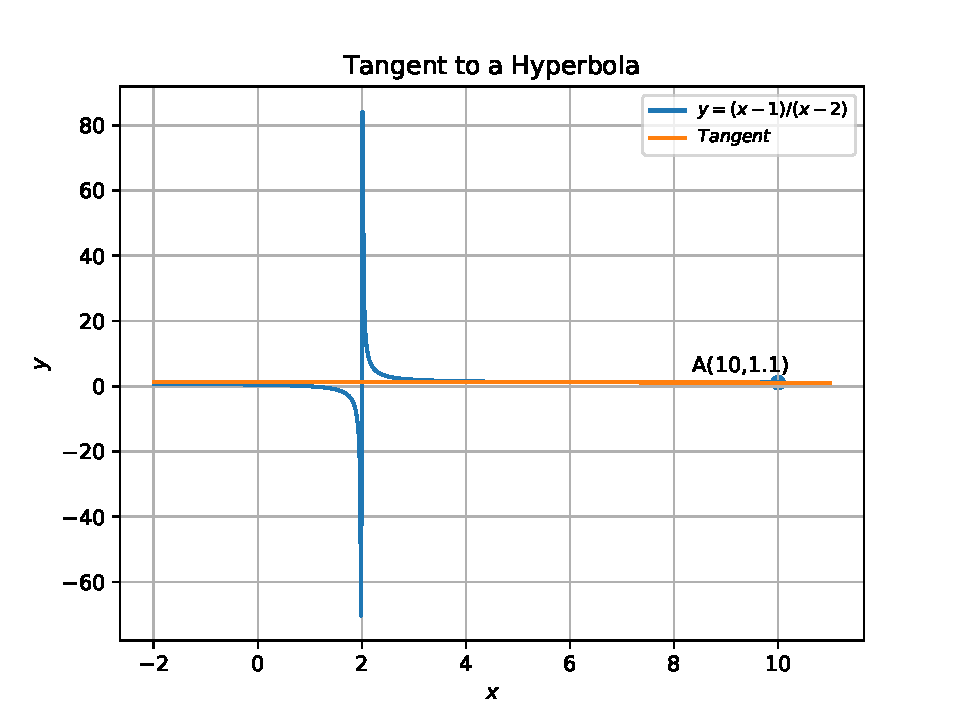
\includegraphics[width=\columnwidth]{chapters/12/6/3/2/figs/problem2.pdf}
	\end{center}
\caption{}
\label{fig:chapters/12/6/3/2/Fig1}
\end{figure}
